\documentclass[aspectratio=169]{beamer}
\usetheme{Madrid}
\usecolortheme{whale}
\usepackage[utf8]{inputenc}
\usepackage[T1]{fontenc}
\usepackage{graphicx}
\usepackage{booktabs}
\usepackage{tabularx}
\usepackage{listings}
\usepackage{xcolor}
\usepackage{tikz}

% ── Color scheme matching the app ──────────────────────────────────────────
\definecolor{edublue}{RGB}{37,99,235}
\definecolor{edubluelight}{RGB}{219,234,254}
\definecolor{edugray}{RGB}{100,116,139}
\setbeamercolor{palette primary}{bg=edublue,fg=white}
\setbeamercolor{palette secondary}{bg=edublue!80,fg=white}
\setbeamercolor{palette tertiary}{bg=edublue!60,fg=white}
\setbeamercolor{palette quaternary}{bg=edublue,fg=white}
\setbeamercolor{structure}{fg=edublue}
\setbeamercolor{block title}{bg=edublue,fg=white}
\setbeamercolor{block body}{bg=edubluelight}
\setbeamertemplate{navigation symbols}{}
\setbeamertemplate{footline}[frame number]

% ── Code style ─────────────────────────────────────────────────────────────
\lstset{
  basicstyle=\ttfamily\small,
  keywordstyle=\color{edublue}\bfseries,
  commentstyle=\color{edugray},
  backgroundcolor=\color{edubluelight},
  frame=single, framerule=0pt,
  breaklines=true
}

% ── Title ─────────────────────────────────────────────────────────────────
\title[EduRAG]{\textbf{EduRAG}}
\subtitle{Serverless AI Knowledge Base\\{\small Milestone 2 — Final Presentation}}
\author{Anna Ostrowska \and Michał Kukla \and Norbert Frydrysiak}
\date{June 2026}
\institute{Serverless \& Cloud Computing}

% ═══════════════════════════════════════════════════════════════════════════
\begin{document}
% ═══════════════════════════════════════════════════════════════════════════

\begin{frame}
  \titlepage
\end{frame}

% ── Agenda ─────────────────────────────────────────────────────────────────
\begin{frame}{Agenda}
  \tableofcontents
\end{frame}

% ═══════════════════════════════════════════════════════════════════════════
\section{Project Overview}
% ═══════════════════════════════════════════════════════════════════════════

\begin{frame}{What is EduRAG?}
  \begin{columns}
    \begin{column}{0.58\textwidth}
      \textbf{EduRAG} is a cloud-native, serverless knowledge base that lets students and researchers \textbf{chat with their study materials} using AI.
      \vspace{0.4cm}

      \begin{block}{Core Idea}
        Upload a textbook PDF\\
        $\Rightarrow$ system indexes it automatically\\
        $\Rightarrow$ ask anything in natural language\\
        $\Rightarrow$ get an answer with \textbf{page citations}
      \end{block}
      \vspace{0.3cm}

      Built entirely on \textbf{Google Cloud Platform} using a fully event-driven, PaaS/Serverless stack.
    \end{column}
    \begin{column}{0.38\textwidth}
      \begin{block}{Key Numbers}
        \begin{tabular}{ll}
          Model & Gemini 1.5 Pro \\
          Embeddings & text-embedding-004 \\
          Chunk size & 1{,}000 chars \\
          Top-K retrieval & 3 chunks \\
          Max PDF size & 50 MB \\
        \end{tabular}
      \end{block}
    \end{column}
  \end{columns}
\end{frame}

% ─────────────────────────────────────────────────────────────────────────
\begin{frame}{User Roles}
  \begin{columns}
    \begin{column}{0.48\textwidth}
      \begin{block}{Student / End User}
        \begin{itemize}
          \item Creates account (username + password)
          \item Uploads PDF textbooks / manuals
          \item Organises documents by \textbf{subject}
          \item Selects which documents to query
          \item Chats with real-time streaming answers
          \item Sees page-level source citations
        \end{itemize}
      \end{block}
    \end{column}
    \begin{column}{0.48\textwidth}
      \begin{block}{Administrator (implicit)}
        \begin{itemize}
          \item No separate admin UI
          \item Infrastructure managed via \textbf{Terraform}
          \item Access through GCP Console
          \item Firestore security rules enforce per-user isolation
        \end{itemize}
      \end{block}
    \end{column}
  \end{columns}
\end{frame}

% ═══════════════════════════════════════════════════════════════════════════
\section{Architecture}
% ═══════════════════════════════════════════════════════════════════════════

\begin{frame}{System Architecture}
  \begin{figure}
    \centering
    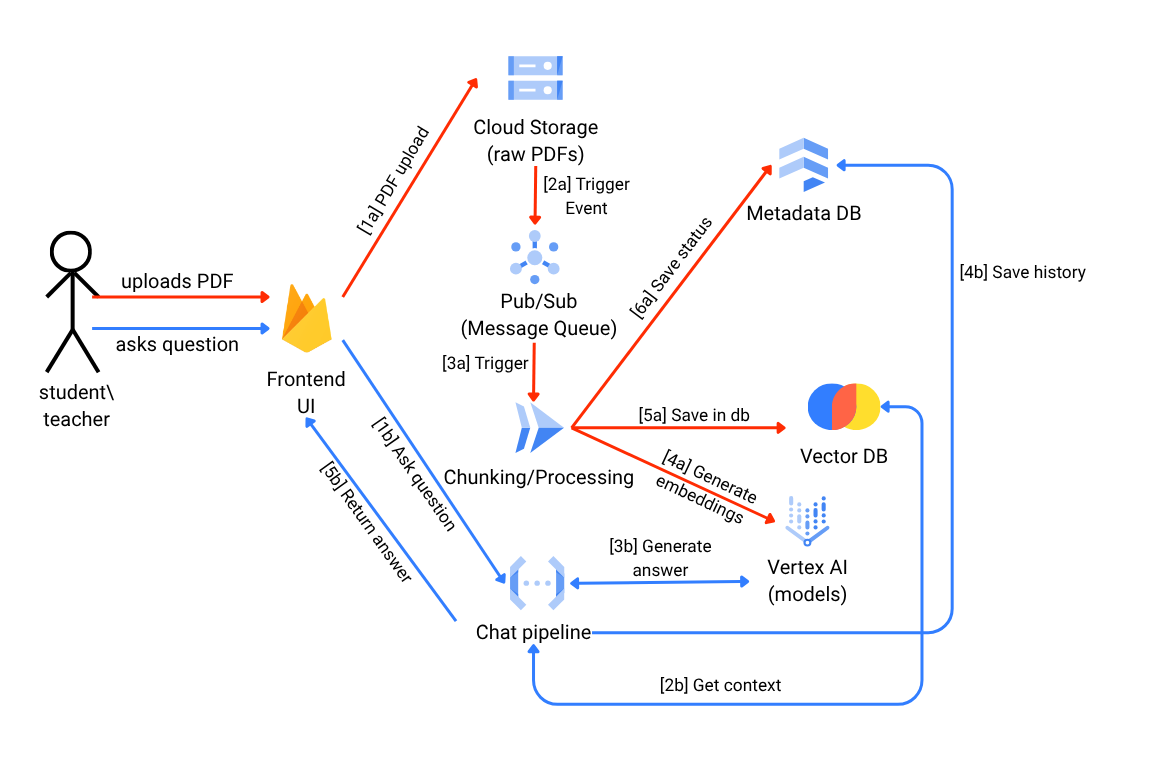
\includegraphics[width=0.92\linewidth]{architecture.png}
    \caption{Two decoupled pipelines: asynchronous ingestion (red) and real-time inference (blue)}
  \end{figure}
\end{frame}

% ─────────────────────────────────────────────────────────────────────────
\begin{frame}{Pipeline 1 — Asynchronous Ingestion}
  \begin{enumerate}
    \item[\textbf{1.}] Frontend requests \textbf{pre-signed URL} from API (bypasses backend for upload)
    \item[\textbf{2.}] PDF uploaded \textbf{directly to GCS} (\texttt{uploads/\{user\}/\{subject\}/\{file\}})
    \item[\textbf{3.}] GCS event triggers \textbf{Pub/Sub} message
    \item[\textbf{4.}] \textbf{Worker (Cloud Run)} receives message:
      \begin{itemize}
        \item Downloads PDF, extracts text with PyPDF
        \item Splits into 1{,}000-char chunks (RecursiveCharacterTextSplitter)
        \item Generates embeddings via \textbf{Vertex AI} \texttt{text-embedding-004}
        \item Stores chunks + vectors in \textbf{ChromaDB}
        \item Updates Firestore status: Downloading $\to$ Chunking $\to$ Vectorizing $\to$ \textbf{Ready}
      \end{itemize}
    \item[\textbf{5.}] Frontend receives real-time status via \textbf{Firestore listener}
  \end{enumerate}
\end{frame}

% ─────────────────────────────────────────────────────────────────────────
\begin{frame}{Pipeline 2 — Real-Time Inference}
  \begin{enumerate}
    \item[\textbf{1.}] User selects documents (checkboxes) and types a question
    \item[\textbf{2.}] \textbf{API (Cloud Run)} receives request with \texttt{question} + \texttt{doc\_ids}
    \item[\textbf{3.}] Question embedded via \textbf{Vertex AI}, similarity search in ChromaDB\\
          (filtered by \texttt{doc\_id} — only selected documents are searched)
    \item[\textbf{4.}] Top-3 most relevant chunks retrieved as context
    \item[\textbf{5.}] Prompt constructed and sent to \textbf{Gemini 1.5 Pro}
    \item[\textbf{6.}] Response \textbf{streamed} back via Server-Sent Events (SSE)\\
          — tokens appear as they are generated, not after full completion
    \item[\textbf{7.}] Frontend renders markdown + displays source citations (filename, page, excerpt)
  \end{enumerate}
\end{frame}

% ─────────────────────────────────────────────────────────────────────────
\begin{frame}{Tech Stack}
  \begin{columns}
    \begin{column}{0.48\textwidth}
      \begin{block}{Backend (GCP)}
        \begin{tabular}{ll}
          \textbf{Compute} & Cloud Run \\
          \textbf{Messaging} & Pub/Sub \\
          \textbf{Storage} & GCS \\
          \textbf{Auth} & Firebase Auth \\
          \textbf{Metadata} & Firestore \\
          \textbf{Vectors} & ChromaDB (CE) \\
          \textbf{LLM} & Vertex AI / Gemini \\
          \textbf{IaC} & Terraform \\
        \end{tabular}
      \end{block}
    \end{column}
    \begin{column}{0.48\textwidth}
      \begin{block}{App / Libraries}
        \begin{tabular}{ll}
          \textbf{API} & Flask + Flask-CORS \\
          \textbf{AI} & LangChain \\
          \textbf{Embeddings} & VertexAIEmbeddings \\
          \textbf{PDF parsing} & PyPDF \\
          \textbf{Frontend} & HTML + Tailwind CSS \\
          \textbf{Hosting} & Firebase Hosting \\
          \textbf{Auth SDK} & Firebase JS SDK \\
        \end{tabular}
      \end{block}
    \end{column}
  \end{columns}
  \vspace{0.3cm}
  \begin{alertblock}{IaaS Exception}
    ChromaDB runs on a \textbf{Compute Engine VM} — the only IaaS component. No native managed vector DB exists on GCP at comparable cost; Vertex AI Vector Search is significantly more expensive.
  \end{alertblock}
\end{frame}

% ═══════════════════════════════════════════════════════════════════════════
\section{Storage}
% ═══════════════════════════════════════════════════════════════════════════

\begin{frame}{Storage Characteristics}
  \renewcommand{\arraystretch}{1.4}
  \begin{tabularx}{\textwidth}{@{} l l l X @{}}
    \toprule
    \textbf{Store} & \textbf{Type} & \textbf{Consistency} & \textbf{Role \& Access Pattern} \\
    \midrule
    Google Cloud Storage
      & Unstructured (blobs)
      & Strong
      & Raw PDFs. Write-once per upload; read-once by the worker. \\
    Firestore
      & NoSQL document (JSON)
      & Strong
      & Per-user document metadata \& processing status. High read+write; drives real-time UI listener. \\
    ChromaDB (Vector DB)
      & Structured (float32 arrays)
      & Eventual
      & Text embeddings. Write-once (on ingestion); read-many (every chat query). \\
    \bottomrule
  \end{tabularx}
  \vspace{0.3cm}
  \begin{block}{Data Volume Estimate (large-scale assumption)}
    1{,}000 users $\times$ 50 docs $\times$ 500 chunks $\times$ 768 floats = \textbf{$\approx$28 GB vectors}. GCS PDFs: up to \textbf{2.5 TB}.
  \end{block}
\end{frame}

% ═══════════════════════════════════════════════════════════════════════════
\section{API Design}
% ═══════════════════════════════════════════════════════════════════════════

\begin{frame}{API Endpoints (REST)}
  \renewcommand{\arraystretch}{1.4}
  \begin{tabularx}{\textwidth}{@{} l l X @{}}
    \toprule
    \textbf{Method} & \textbf{Endpoint} & \textbf{Description} \\
    \midrule
    GET  & \texttt{/generate-upload-url} & Returns pre-signed GCS URL. Params: \texttt{filename}, \texttt{subject}. Creates Firestore doc. Requires auth. \\
    POST & \texttt{/ask}                 & SSE streaming chat. Body: \texttt{question}, \texttt{doc\_ids[]}. Returns token stream + sources. Requires auth. \\
    \bottomrule
  \end{tabularx}
  \vspace{0.4cm}
  \begin{columns}
    \begin{column}{0.48\textwidth}
      \begin{block}{Authentication}
        All endpoints require\\
        \texttt{Authorization: Bearer \{Firebase ID token\}}
      \end{block}
    \end{column}
    \begin{column}{0.48\textwidth}
      \begin{block}{SSE Response format}
        \texttt{data: \{"token": "...\}}\\
        \texttt{data: \{"token": "...\}}\\
        \texttt{data: \{"sources": [...], "done": true\}}
      \end{block}
    \end{column}
  \end{columns}
\end{frame}

% ═══════════════════════════════════════════════════════════════════════════
\section{SLA / SLO / SLI}
% ═══════════════════════════════════════════════════════════════════════════

\begin{frame}{SLA / SLO / SLI}
  \begin{block}{SLA — Service Level Agreement (commitment to users)}
    99.9\% uptime for the Chat UI and Inference API (backed by GCP managed services SLA).
  \end{block}
  \vspace{0.3cm}
  \begin{block}{SLOs — Service Level Objectives}
    \begin{itemize}
      \item \textbf{Inference latency:} 95\% of \texttt{/ask} requests return the first streamed token in $<\!2$s
      \item \textbf{Ingestion throughput:} 99\% of PDFs ($<$50 MB) fully vectorised within 3 minutes of upload
      \item \textbf{Availability:} Chat API error rate $<$ 0.1\% over any 30-day window
    \end{itemize}
  \end{block}
  \vspace{0.3cm}
  \begin{block}{SLIs — Service Level Indicators (how we measure)}
    \begin{itemize}
      \item \textbf{Time-to-first-token:} Cloud Run request latency to first SSE chunk (Cloud Monitoring)
      \item \textbf{Ingestion duration:} Firestore timestamp delta between \textit{Uploading} and \textit{Ready} status
      \item \textbf{Error rate:} HTTP 5xx responses / total requests (Cloud Run metrics)
    \end{itemize}
  \end{block}
\end{frame}

% ═══════════════════════════════════════════════════════════════════════════
\section{Large-Scale Assumptions}
% ═══════════════════════════════════════════════════════════════════════════

\begin{frame}{Large-Scale Assumptions}
  \begin{columns}
    \begin{column}{0.48\textwidth}
      \begin{block}{Load model}
        \begin{tabular}{ll}
          Registered users    & 10{,}000       \\
          Concurrent users    & 500            \\
          Docs per user       & up to 50       \\
          Doc size            & up to 50 MB    \\
          Chat requests/min   & 1{,}000 QPS    \\
          Uploads/hour        & 200            \\
        \end{tabular}
      \end{block}
    \end{column}
    \begin{column}{0.48\textwidth}
      \begin{block}{Why it scales}
        \begin{itemize}
          \item \textbf{Cloud Run} scales to 0 when idle; scales out automatically under load (no fixed servers)
          \item \textbf{Pub/Sub} buffers upload bursts; worker processes them asynchronously
          \item \textbf{Direct-to-GCS upload} bypasses the API entirely for file transfer
          \item \textbf{Firestore} handles thousands of concurrent listeners natively
        \end{itemize}
      \end{block}
    \end{column}
  \end{columns}
  \vspace{0.3cm}
  \begin{alertblock}{Bottleneck}
    ChromaDB on a single Compute Engine VM is the main scalability constraint — horizontal sharding would require a managed vector DB (Vertex AI Vector Search).
  \end{alertblock}
\end{frame}

% ═══════════════════════════════════════════════════════════════════════════
\section{Key Features}
% ═══════════════════════════════════════════════════════════════════════════

\begin{frame}{Key Features Implemented}
  \begin{columns}
    \begin{column}{0.48\textwidth}
      \textbf{Infrastructure}
      \begin{itemize}
        \item Full Terraform IaC (Cloud Run, GCS, Pub/Sub, Firestore, IAM, Artifact Registry)
        \item Event-driven architecture (GCS $\to$ Pub/Sub $\to$ Worker)
        \item Containerised services (Docker + gunicorn)
      \end{itemize}
      \vspace{0.2cm}
      \textbf{Security}
      \begin{itemize}
        \item Firebase Auth (Google SSO + username/password)
        \item Per-user data isolation (Firestore \& ChromaDB filters)
        \item Pre-signed URLs — PDFs never pass through backend
      \end{itemize}
    \end{column}
    \begin{column}{0.48\textwidth}
      \textbf{User Experience}
      \begin{itemize}
        \item Subject / folder organisation (like Google Drive)
        \item Per-document checkboxes — choose which docs to query (like NotebookLM)
        \item Streaming responses (SSE) — tokens appear instantly
        \item Page-level source citations with text excerpts
        \item Markdown rendering (bold, lists, code blocks)
        \item Real-time processing status (Firestore listener)
      \end{itemize}
    \end{column}
  \end{columns}
\end{frame}

% ═══════════════════════════════════════════════════════════════════════════
\section{Live Demo}
% ═══════════════════════════════════════════════════════════════════════════

\begin{frame}{Live Demo}
  \begin{center}
    {\Huge 🎬}\\[0.5cm]
    {\Large \textbf{Live Demo}}\\[0.4cm]
    \begin{block}{Demo Flow}
      \begin{enumerate}
        \item Register a new account (username + password)
        \item Create subject folder (e.g. \textit{Cloud Computing})
        \item Upload a PDF textbook
        \item Watch real-time processing status (Downloading $\to$ Ready)
        \item Select the document and ask a question
        \item Show streaming answer with source citations
        \item Deselect document, ask again — show empty context response
      \end{enumerate}
    \end{block}
  \end{center}
\end{frame}

% ═══════════════════════════════════════════════════════════════════════════
\section{Summary}
% ═══════════════════════════════════════════════════════════════════════════

\begin{frame}{Summary}
  \begin{columns}
    \begin{column}{0.58\textwidth}
      \begin{block}{What we built}
        A production-ready, serverless RAG knowledge base on GCP with:
        \begin{itemize}
          \item Decoupled async ingestion + real-time inference
          \item Multi-user auth with document isolation
          \item Subject organisation + selective doc querying
          \item Streaming AI responses with citations
          \item Complete IaC with Terraform
        \end{itemize}
      \end{block}
      \vspace{0.3cm}
      \begin{alertblock}{One IaaS component}
        ChromaDB on Compute Engine VM — justified by cost vs.\ Vertex AI Vector Search.
      \end{alertblock}
    \end{column}
    \begin{column}{0.38\textwidth}
      \begin{block}{Requirements}
        \begin{tabular}{lc}
          UI                & \checkmark \\
          Storage           & \checkmark \\
          Terraform         & \checkmark \\
          Large-scale       & \checkmark \\
          PaaS/Serverless   & \checkmark* \\
          Auth              & \checkmark \\
          Real-time updates & \checkmark \\
          Streaming         & \checkmark \\
        \end{tabular}
        \small{*except ChromaDB VM}
      \end{block}
    \end{column}
  \end{columns}
\end{frame}

% ─────────────────────────────────────────────────────────────────────────
\begin{frame}
  \begin{center}
    {\Huge \textbf{Q\&A}}\\[0.6cm]
    {\large Thank you!}\\[0.4cm]
    \small
    Anna Ostrowska \quad Michał Kukla \quad Norbert Frydrysiak
  \end{center}
\end{frame}

\end{document}
